\chapter{Model Design} 

\section{Gravity Model}
As discussed in section~\ref{section:lit-review}, the Gravity model is still the standard approach to estimating OD trip distribution matrices. Its simplicity and low computational complexity makes it attractive to modellers. I This chapter, a gravity model for the combined zone system is presented. In modelling, it is always a good idea to develop the simplest model first. Firstly, it may be good enough, and a more complex model not required. Secondly, the errors in simpler models can aid the development of more complicated models. As such, this model will then be used as a baseline to compare the destination choice models presented in section~\ref{section:destination-choice}

\subsection{Design}
The gravity model is singly constrained on the origin, with the size of each zone being the sum of population and employment. The gravity model is specified as followed:

$$ 
T_{ij} = \frac{A_j \cdot e^{-k \cdot d_{ij}}}{\sum_{all zones} A_j \cdot e^{-k \cdot d_{ij}}} \cdot P_i $$

Where \\
$T_{ij}$ is the number of trips between zones $i$, $j$. \\
$P_j$ is the number of trips produced in origin zone $i$.\\
$A_j$ is the attraction at destination zone $j$.\\
$k$ is the impedance factor, calibrated with the average trip distance.\\
$d_{ij}$ is the distance between zones $i$, $j$.\\


\subsection{Calibration}
A separate model was created for each trip purpose, and calibrated to match the expected average trip distance $\bar{d}$, calculated from the trip distances recorded in the TSRC, to within 1\%. The results of the calibration are presented in table~\ref{table:gravity-calibration}. The average observed trip distance is $\bar{d}$, the average predicted trip distance $d$, and the impedance factor $k$. As measurements of error, the root mean square error (RMSE) and model correlation ($r^2$) are provided.

\begin{table}[H]
\centering
\caption{Gravity Model Calibration}
\label{table:gravity-calibration}
\begin{tabular}{@{}lllllll@{}}
\toprule
Model & Trips & $\bar{d}$ & $d$ & $k$ & RMSE & $r^2$ \\ \midrule
   Business  & 34,229.43  &     244     &  242.92   & 0.0002 & 57.48  & 0.33  \\
   Leisure   & 83,357.94  &     149     &  150.79   & 0.0016 & 93.43  & 0.36  \\
   Visit     & 129,843.18 &     163     &  161.00   & 0.0013 & 104.45 & 0.40  \\ \bottomrule
\end{tabular}
\end{table}


\subsection{Results}
Figure~\ref{fig:gravity-residuals} presents an error plot, with the observed trips on the x axis, and difference between the observed and predicted on the y axis. While the three purposes cannot be compared with each other, due to the differing sample sizes, it is clear that all three models have serious errors, and are almost unusable. The predicted values should fall roughly above and below the dotted line. There is a definite pattern in the observed data, indicating that important OD pairs, ones with large numbers of trips, are strongly underestimated. The calibration attempts to fit the many OD pairs with smaller number of trips to fit the observed average trip distance. However, this comes at the expense of model accuracy for large, important connections.

\begin{figure}[H]
\centering
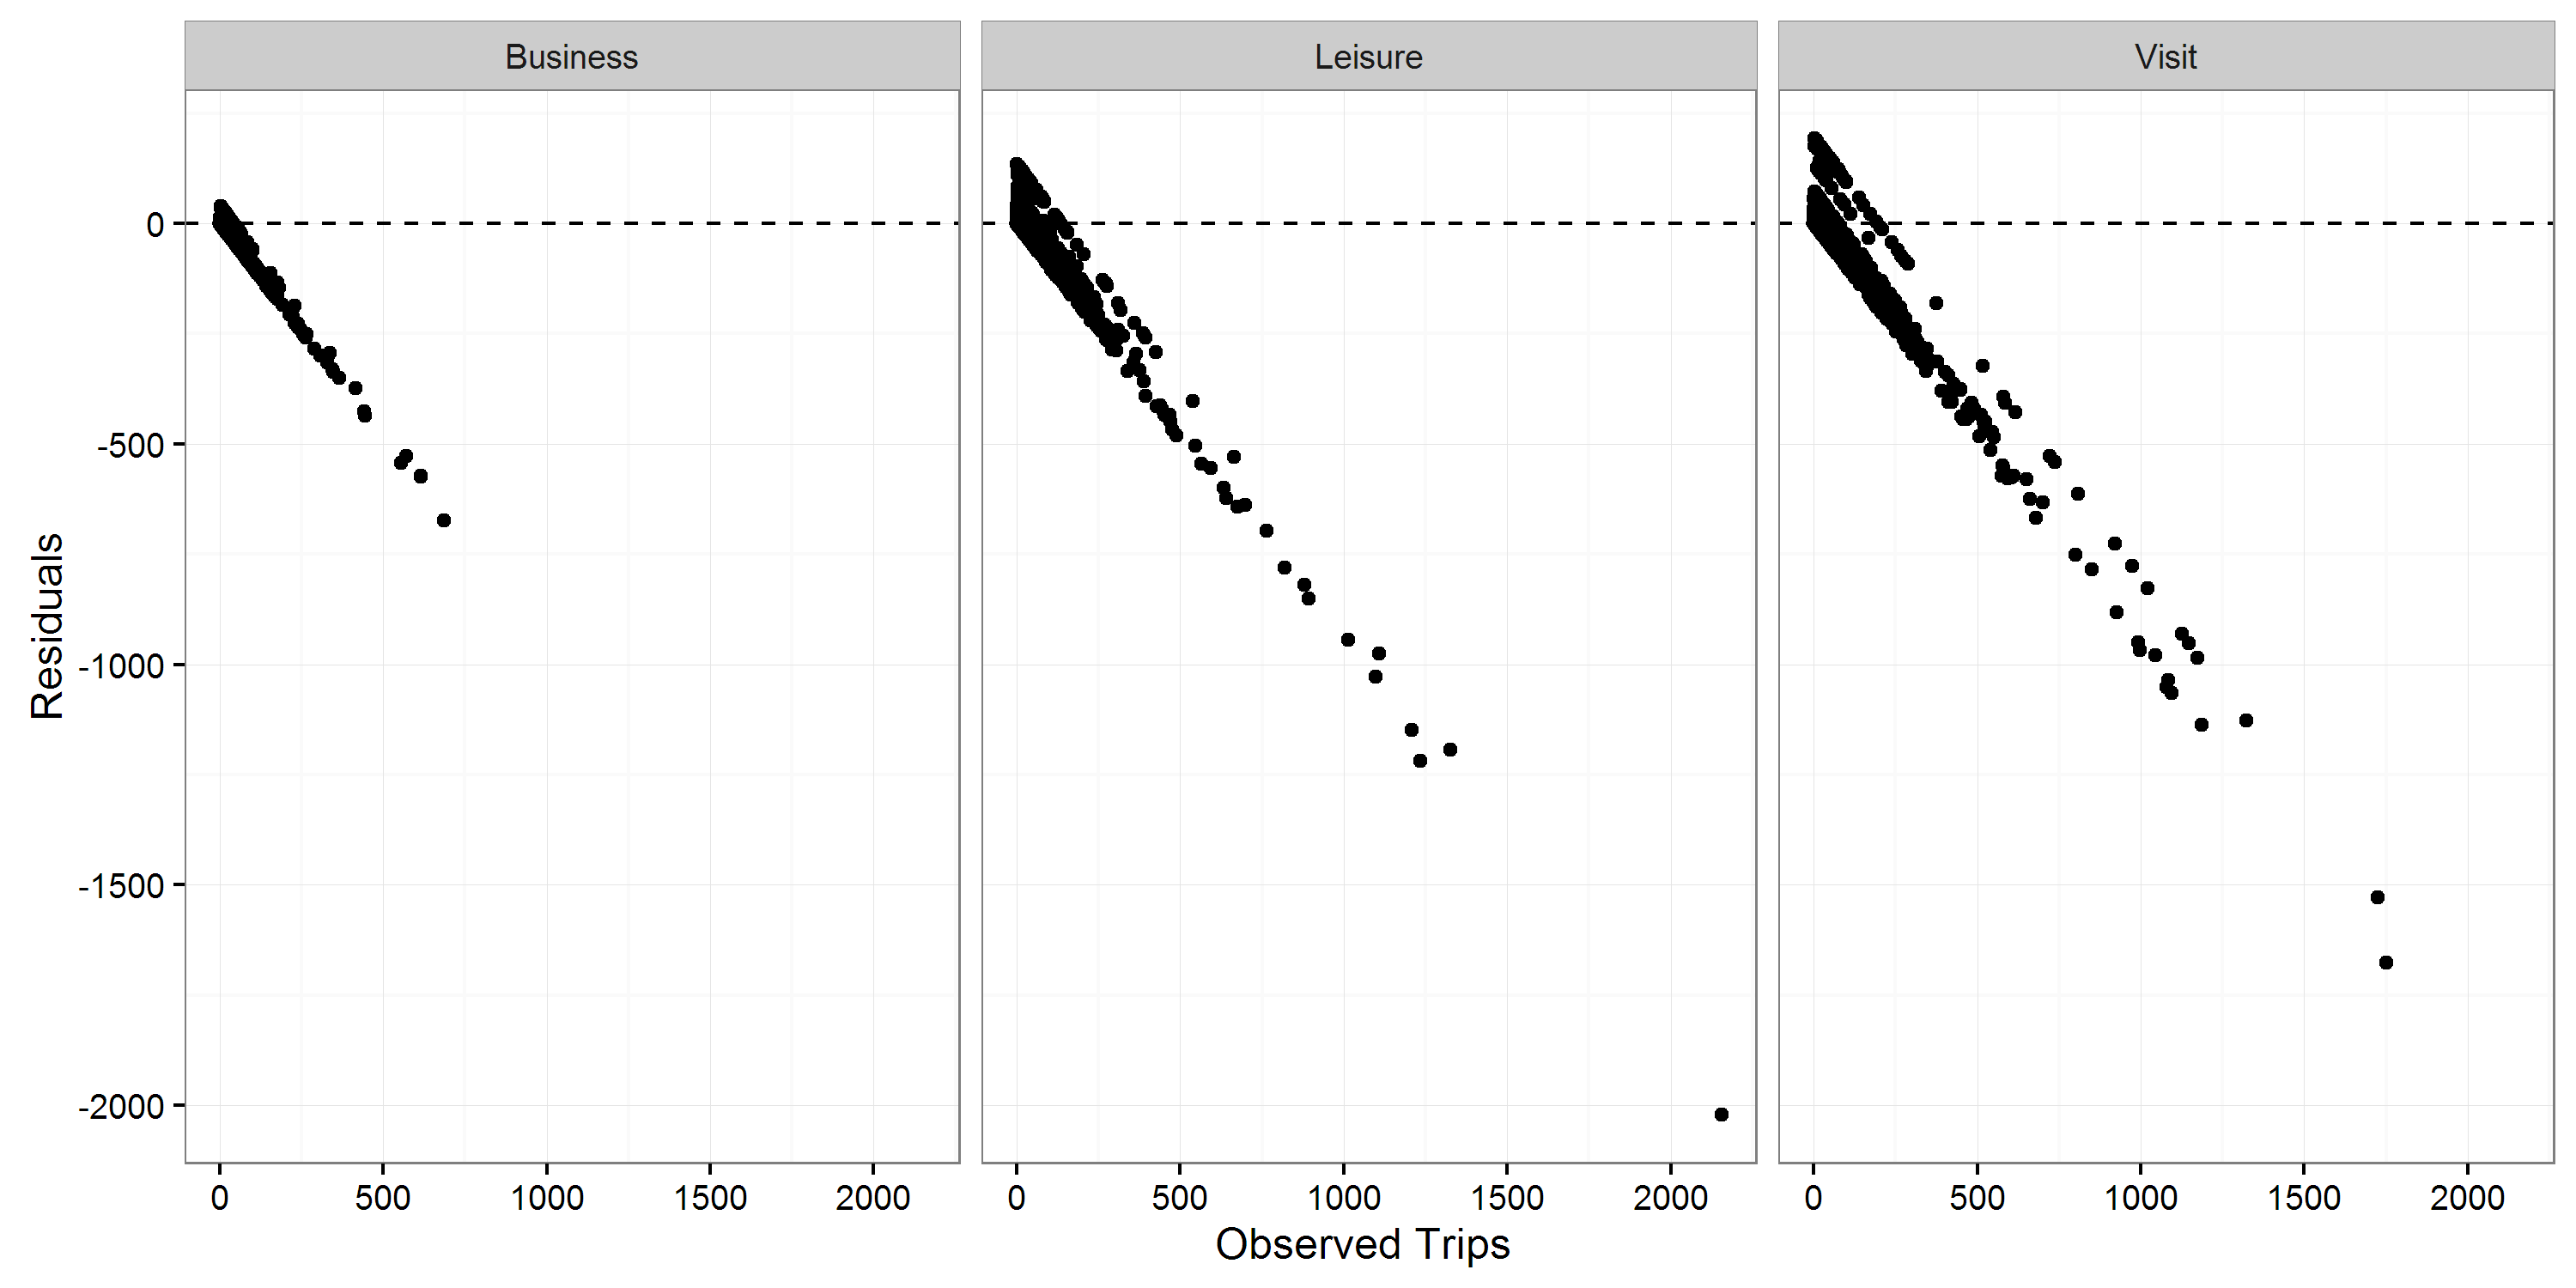
\includegraphics[width=\textwidth]{gravity_model_residuals}
\caption{Gravity model errors by observed trip count for OD pairs by trip purpose}
\label{fig:gravity-residuals}
\end{figure}

Figure~\ref{fig:gravity-errors} gives a better indication of how the model fits these important zones. On the x axis is the absolute error $|x - E(x)|$, and on the y axis, a variant of the relative error, which we call maximum relative error is plotted. 

$$\frac{|x-E(x)|}{\min(x, E(x))}$$

This error metric was chosen over the standard relative error $\frac{|x-E(x)|}{E(x)}$ as it treats over and underestimations equally. When the relative error is used, only one term, $E(x)$ is in the denominator, meaning that large underestimations produce very small relative errors, reducing the visibility of such errors in the chart. Large y values are only of concern when the x value, namely absolute error, is also large.

\begin{figure}[H]
\centering
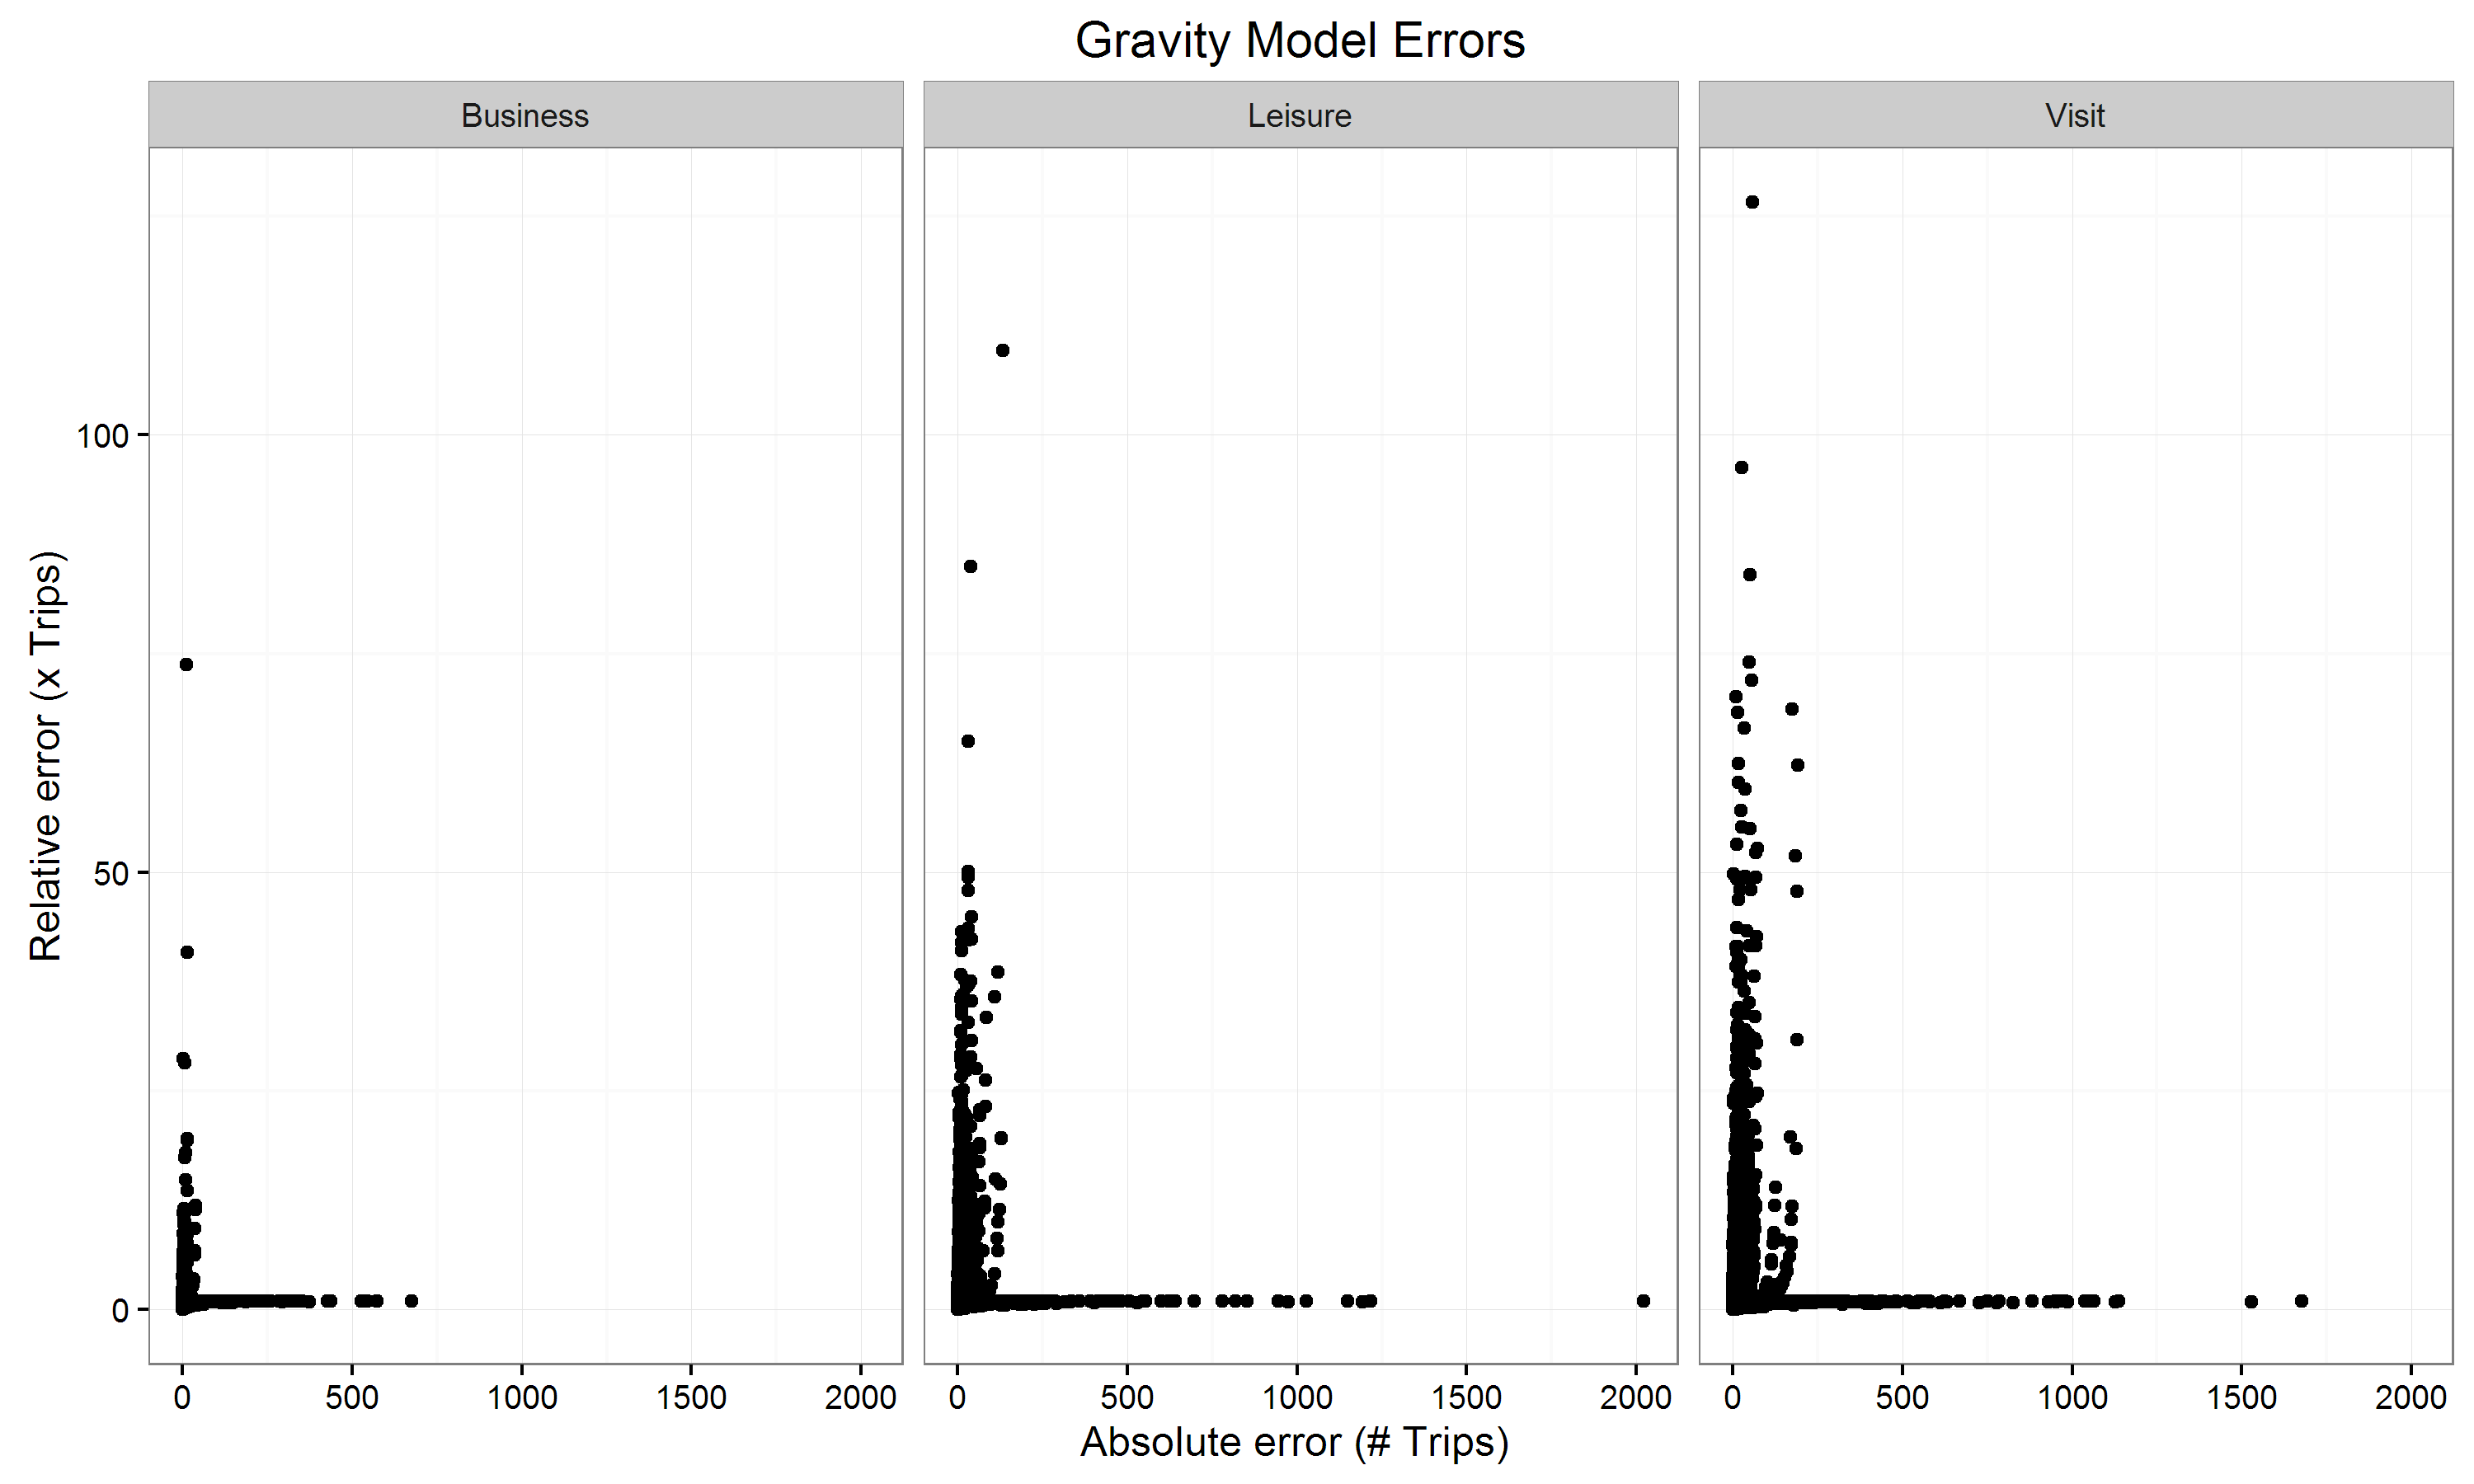
\includegraphics[width=\textwidth]{gravity_model_errors}
\caption{Maximum relative error chart for OD pairs by trip purpose}
\label{fig:gravity-errors}
\end{figure}

Large outliers for all three trip purposes in figure~\ref{fig:gravity-errors}. The size of these errors even obscures the also important errors closer to the origin. The points along the x axis indicate that some OD pair estimations are off by over 1000 trips. 

Investigating leisure trips, significant outliers are visible. A clear weakness of the gravity model can be seen by further examining some of these outliers. The number of leisure trips originating from zones in the Toronto region to tourist destinations just outside of Toronto, such as Niagara Falls and Muskoka are strongly underestimated. By its nature, the gravity model is limited in how it can model such zone interactions, as it only takes into account one attraction factor and one impedance factor.

The propensity for leisure travellers to visit destinations with tourist attractions is clearly determined by factors other than the population and employment of the destination. The multinomial logit model of destination choice discussed in the next section adds such factors, and explores how they can be modelled.

\chapter{Destination Choice Model}
\label{section:destination-choice}

\section{Estimation}
\subsection{Socio-economic Variables}
\subsection{Origin-Destination Interactions}
\subsection{Incorporating LBSN Data}
\subsection{Model Subsets}
\paragraph{Seasons}
\paragraph{Income Strata}
\subsection{Final Model}


